
\documentclass{article}
\usepackage{hyperref}
\usepackage{graphicx}
\begin{document}

\title{LabWork3}
\section{Introduction}

Nathan Choukroun labwork 3

Cuda programming of greyscale function

\section{Code to run}

\href{hpc_lab3_greyscale.ipynb}{Labwork notebook}

\section{Results}

To run a function that takes as in put an image and transform it to a greyscale image, we will run a cuda function that utilizes the gpu cores to parralelize the computation for each pixel color. We simulate a picture with a random 3D array of color value between 0 and 255. The kernel function will calculate the average value of the three colors and return it to the whole pixel. This will give a grey color to each pixel and be repeted on the whole matrix. The new matrix is then sent to the host to display it as an image. 

To measurate the impact of the block size in the computation time, we added a timer around the running of the kernel. We also loop the process for each block size to graph it and compare the time it takes. 

We see that he first value that run is always higher than the rest. Only for the graph I changed it to 0 so the range of the other values is more precise. We can note that the first computation react differently. 

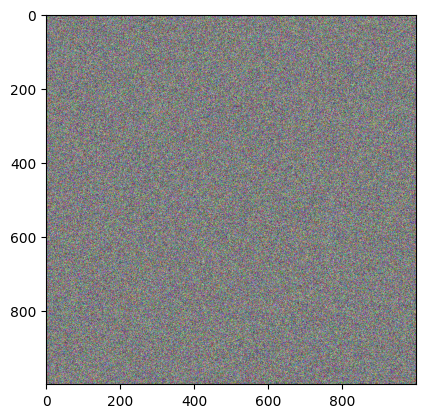
\includegraphics[width=0.4\textwidth]{pixelGridColor.png}
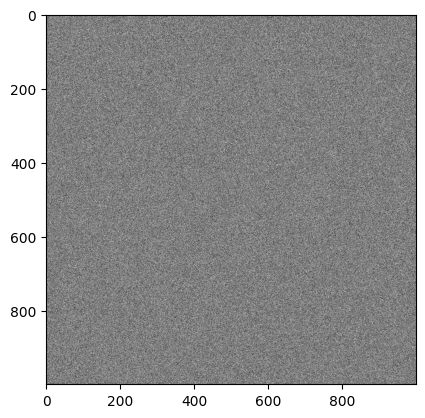
\includegraphics[width=0.4\textwidth]{pixelGrid.png}


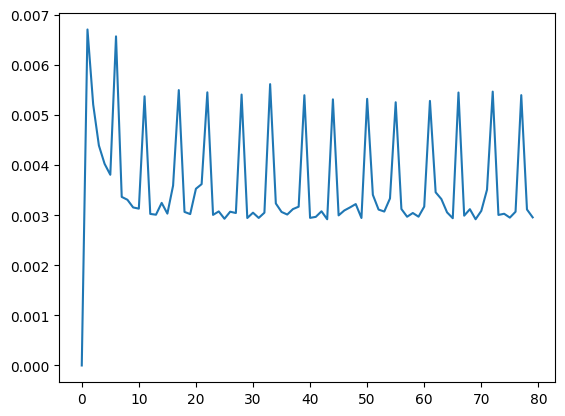
\includegraphics[width=0.4\textwidth]{graphBlockSize.png}


Time to run is: 
``[0.17851758 0.00670314 0.00520658 0.00438881 0.0040226  0.00380468 0.00656581 0.00336313 0.00330591 0.00315285 0.00312901 0.00537014 0.00302362 0.00300789 0.00324368 0.00302958 0.00358891 0.00549388 0.00306368 0.00302005 0.00352526 0.00361776 0.00544906 0.00300431 0.00307345 0.00292706 0.00306749 0.00304174 0.00540447 0.00294209 0.00304818 0.00294375 0.00304818 0.00561261 0.00323248 0.00306296 0.00301147 0.00311995 0.00316811 0.0053916  0.00294471 0.00296474 0.00307608 0.00291705 0.0053091  0.0029943  0.00309253 0.00315356 0.00322008 0.00294232 0.00531936 0.00340414 0.00311017 0.00307107 0.00333238 0.00525117 0.00312185 0.00296736 0.00304198 0.00296831 0.00316954 0.00527811 0.00345492 0.00332022 0.00305438 0.00293756 0.00544548 0.00298858 0.0031178  0.00291729 0.00308466 0.00350666 0.0054636  0.00300312 0.00302672 0.00294971 0.00306726 0.00539327 0.00311232 0.00295496]''


\end{document}